\documentclass[12pt,a4paper]{article}

\usepackage[utf8]{inputenc}
\usepackage[spanish]{babel}
\usepackage[T1]{fontenc}
\usepackage[backend=biber, style=ieee]{biblatex}
\usepackage[a4paper, total={6.5in, 8.75in}]{geometry}\usepackage[most]{tcolorbox}
\usepackage{booktabs}
\usepackage{float}
\usepackage{caption}
\usepackage{amsmath,amsfonts,amssymb}
\usepackage{csquotes}
\usepackage{fancyhdr}
\usepackage{tocloft}
\usepackage{graphicx}
\usepackage{hyperref}
\usepackage{geometry}
\usepackage{wrapfig}
\usepackage{placeins}
\usepackage{tikz}
\usepackage{lipsum}
\usepackage{multicol}
\usepackage{booktabs}
\usepackage{tabularx}
\usepackage{colortbl}

% -------------------------------------------------
\usepackage{tgadventor}
\renewcommand*\familydefault{\sfdefault}
\geometry{left=2cm,right=2cm,top=2cm,bottom=2cm}

% Bib
\addbibresource{referencias.bib}

\hypersetup{
    colorlinks=true,
    linkcolor=blue,     
    citecolor=blue,     
    urlcolor=blue       
}

\defbibheading{bibliography}[\refname]{%
  \subsection{#1}%
  \markboth{#1}{#1}}


% -------------------------------------------------
% Comndos
\renewcommand{\headrulewidth}{0.4pt}
\renewcommand{\footrulewidth}{0.4pt}
\renewcommand{\cftsecleader}{\cftdotfill{\cftdotsep}}

\newcommand{\nProyecto}{AdmisiónTEC}
\newcommand{\nVersion}{Versión 1.0}
\newcommand{\nSponsor}{Instituto Tecnológico de Costa Rica}
\newcommand{\nSupervisor}{Ericka Solano Fernández}

\newtcolorbox{conceptbox}[2][]{%
    colback=teal!5!white,
    colframe=teal!75!black,
    fonttitle=\bfseries,
    colbacktitle=teal!85!black, 
    enhanced,
    attach boxed title to top left={yshift=-2mm, xshift=2mm},
    title=#2,
    #1
}

\newcommand{\concept}[2]{%
    \begin{conceptbox}{#1}
    #2
    \end{conceptbox}
}

% -------------------------------------------------
% Colores
\definecolor{lightgray}{gray}{0.9}

% -------------------------------------------------

\begin{document}

\begin{minipage}{0.3\textwidth}
  \begin{tikzpicture}
      \fill[black] (0,0) rectangle (0.8\linewidth, 0.86\paperheight);
  \end{tikzpicture}
\end{minipage}
\hfill
\begin{minipage}{0.7\textwidth}
  
  \textbf{\Huge Diseño de Arquitectura de}\\
  \textbf{\Huge Software}\\[0.8cm]
  \textbf{\LARGE \nProyecto}\\[0.3cm]
  \textbf{\Large \nVersion}\\[0.2cm]
  12 de Octubre 2023
  
  \vspace{1.2cm}
  \large
  \textbf{Sponsor} \\
  \nSponsor \\
  \textbf{Supervisora} \\
  \nSupervisor

  \vspace{2cm}
  
  \begin{multicols}{2}
      \large
      \textbf{Miembros del equipo}\\
      Hansol Antay\\
      Elon Musk\\
      
      \columnbreak
      
      \textbf{Contacto}\\
      rostrhan@outlook.com\\
      elon@musk.com
  \end{multicols}
  
\end{minipage}

\vfill

\newpage

\tableofcontents

\newpage

\section*{Historial de versiones}

\begin{table}[h!]
  \centering
  \begin{tabular}{l c p{10cm} l}
      \rowcolor{lightgray}
      Fecha & \# & Descripción & Autor \\
      \midrule
      12/08/2023 & 
      1.0 & 
      Creación del documento base, es una entrega preliminar. & 
      H. Antay \\
      \bottomrule
  \end{tabular}
  \label{tab:historialversiones}
\end{table}

\section{Introducción}

\subsection{Propósito}

Este proyecto tiene como propósito principal brindar al ITCR una herramienta en línea que lo ayude a gestionar los procesos administrativos que conllevan el examen de admisión de la institución. Con este documento en particular se busca brindar una visión inicial del sistema modelando y detallando sus componentes, interacciones y funcionalidades principales.

\subsection{Alcance}

En este documento se va a cubrir las especificaciones arquitectónicas del sistema de solicitudes para el examen de admisión del ITCR. En este se va a cubrir la interacción con la bases de datos, modelado de clases, especificación del proceso de registro de solicitantes y el proceso de simulación y notificación de notas.

\subsection{Definiciones, acrónimos y abreviaciones}

\begin{itemize}
  \item \textbf{TEC:} Tecnológico de Costa Rica.
  \item \textbf{ITCR:} Instituto Tecnológico de Costa Rica.
  \item \textbf{UML:} Unified Modeling Language, significa lenguaje de modelado unificado. \cite{OMG2017}
  \item \textbf{MVC:} Patrón de diseño de software Modelo-Vista-Controlador.
\end{itemize}

\printbibliography
  
\section{Representación arquitectónica}

En la especificación del documento se indica que al momento en el que se registra un usuario este va a tener que indicar la carrera en la que desea ingresar. Se consideró algo poco práctico por lo que esta propuesta tendrá un enfoque diferente.

Considerando que una persona puede realizar varios exámenes de admisión se planteó que el registro se hiciera sin la necesidad de indicar la carrera directamente. Se hace un registro ``común'', y ya una vez ingresado en el sistema el usuario podrá optar por realizar un examen de admisión según sea habilitado.

Esta propuesta sería más práctica. Pensando más a futuro en la evolución de la aplicación, el usuario podría seleccionar distintas fechas/horas para realizar la aplicación del examen, podría consultar de forma más rápida los resultados o estados de los exámenes de admisión, gestionar de forma más directa los pagos para poder realizar el examen e incluso se podría escalar y considerar exámenes de otras universidades.
El diagrama de componentes de detalla a continuación:
\begin{figure}[H]
  \centering
  \frame{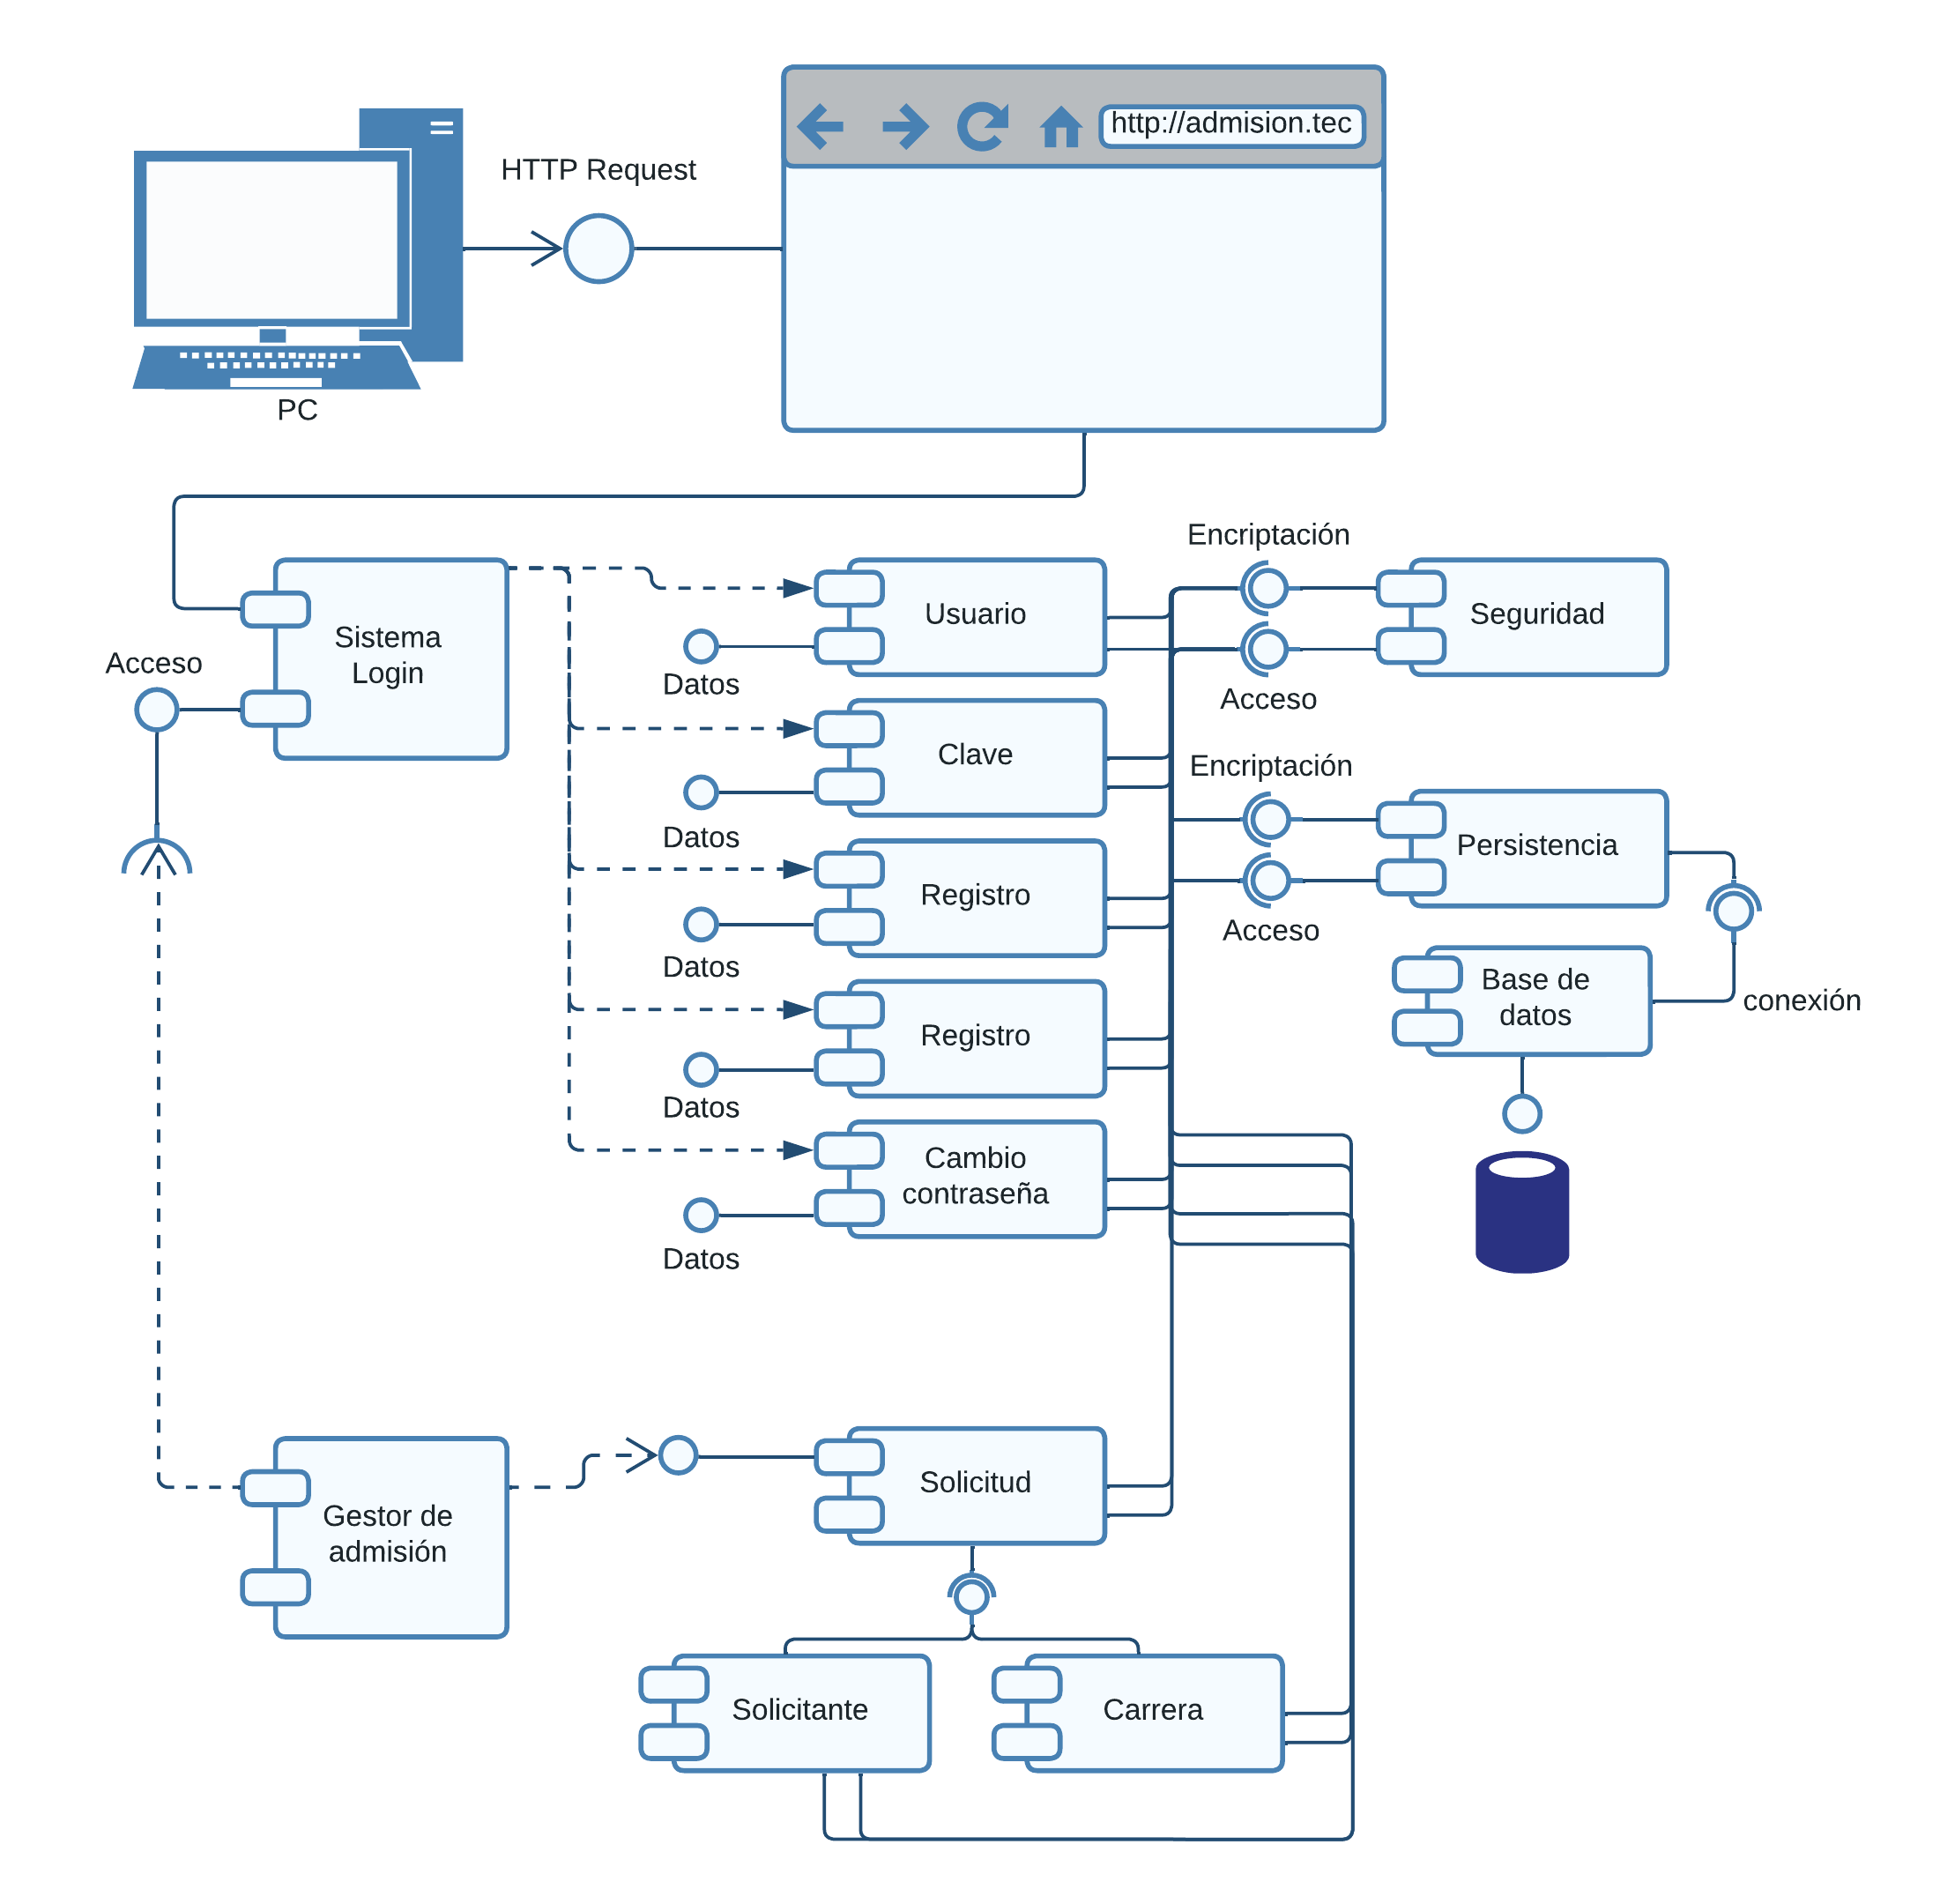
\includegraphics[width=\textwidth]{./img/componentesDiag.png}}
  \caption{Diagrama de componentes}
  \label{fig:diagComponentes}
\end{figure}

\section{Objetivos y restricciones de la arquitectura}

\subsection{Objetivos}

\begin{itemize}
  \item \textbf{Escalabilidad.} Como se mencionó anteriormente, se podría integrar fácilmente más carreras e incluso instituciones que quieran hacer uso de este sistema.
  \item \textbf{Usabilidad.} Debe ser un sistema fácil de utilizar, con una interfaz sencilla pero agradable para los usuarios finales.
  \item \textbf{Seguridad.} La información debe manejarse de forma segura, todos los datos estarán cifrados y descifrados de forma segura.
  \item \textbf{Persistencia de datos.} Todos los datos deben almacenarse de forma persistente en una base de datos.
  \item \textbf{Disponibilidad.} El sistema deberá estar disponible en momentos de alta demanda. Considerando en períodos de tiempo en dónde se anuncia o promociona las solicitudes para la realización del examen de admisión y cuando se brindarán los resultados de los mismos.
\end{itemize}

\subsection{Restricciones}
\begin{itemize}
  \item Todos los usuarios deberán identificarse para poder acceder a la plataforma. Este mecanismo debe ser completamente seguro.
  \item Los administradores podrán modificar los datos de \textit{nota mínima de admisión} y la \textit{cantidad máxima de gente admisible} en las carreras pero respetando restricciones.
  \item Los datos de solicitudes deberán enviarse de forma encriptada a la base de datos utilizando mecanismos de seguridad.
  \item El sistema deberá implementarse haciendo uso del patrón de diseño Modelo-Vista-Controlador.
\end{itemize}

\section{Vista casos de uso}

En esta sección veremos los casos de uso más relevantes para el sistema, primero definiremos textualmente estos casos de uso y los mostraremos con su respectivo diagrama.

\subsection{Caso de uso: Inicio de sesión}

\begin{tcolorbox}[colback=white, colframe=black, rounded corners]
  {\Large \textbf{Caso de uso: Inicio de sesión}} \\
  {\large Actor: Usuario} \vspace*{0.5cm} \\
  {{\large \textbf{Precondiciones}} \\
  1. El usuario está registrado. \\
  2. El usuario ingresó a la página de inicio de sesión.
  } \vspace*{0.5cm} \\
  {{\large \textbf{Flujo principal}} \\
  1. El usuario ingresa usuario y contraseña. \\
  2. El sistema valida la información. \\
  3. Si la información es válida, se permite el acceso y se redirecciona a la página principal.
  } \vspace*{.5cm} \\
  {{\large \textbf{Flujo alternativo}} \\
  2a. Información del usuario incorrecta.
  \begin{itemize}
    \item Se muestra un mensaje de error.
    \item El usuario puede volver a intentar.
  \end{itemize}
  2b. El usuario indica que olvidó la contraseña.
  \begin{itemize}
    \item El usuario hace clic en la opción ``olvidé mi contraseña''.
    \item Se realiza el caso de uso \textbf{Recuperación de cuenta}.
  \end{itemize}
  }
\end{tcolorbox}

\begin{figure}[H]
  \centering
  \frame{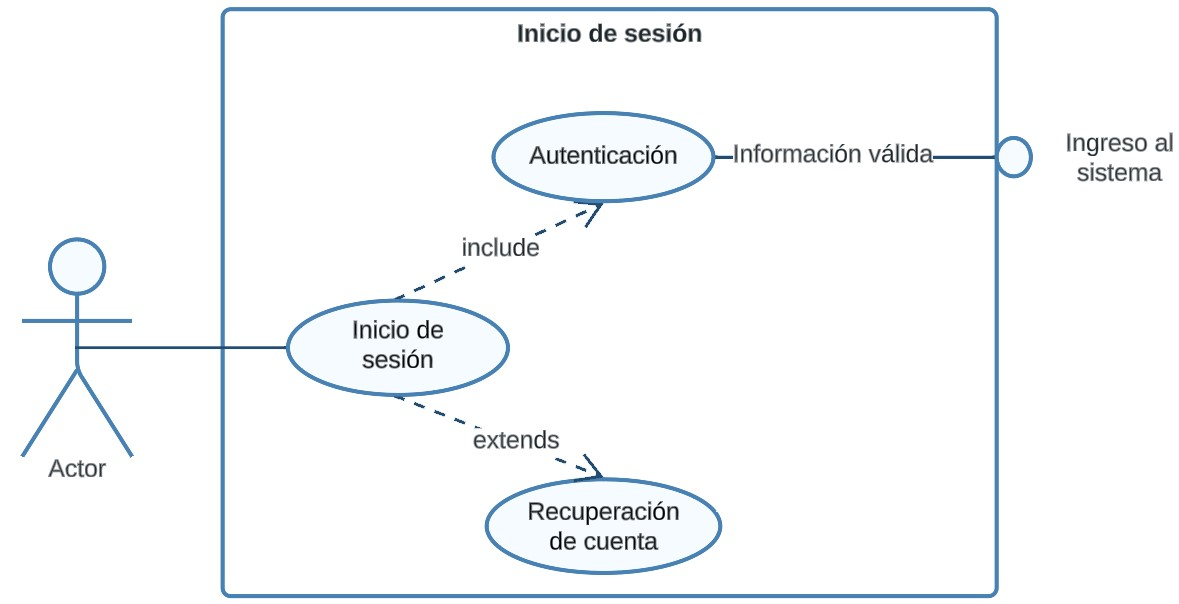
\includegraphics[width=\textwidth]{./img/casousoLogin.jpg}}
  \caption{Diagrama de caso de uso: Inicio de sesión}
  \label{fig:diagusoLogin}
\end{figure}

\subsection{Caso de uso: Realizar solicitud de examen}

\begin{tcolorbox}[colback=white, colframe=black, rounded corners]
  {\Large \textbf{Caso de uso: Solicitud de examen de admisión}} \\
  {\large Actor: Usuario registrado} \vspace*{0.5cm} \\
  {{\large \textbf{Precondiciones}} \\
  1. El usuario ha ingresado al sistema. \\
  2. El usuario no ha solicitado un examen de admisión en el año en curso.
  } \vspace*{0.5cm} \\
  {{\large \textbf{Flujo principal}} \\
  1. El usuario navega a la sección de ``Examen de Admisión''. \\
  2. El sistema muestra distintas fechas/horas disponibles para realizar el examen. \\
  3. El usuario selecciona una fecha/hora que le convenga. \\
  4. El usuario hace clic en el botón ``Realizar solicitu''. \\
  5. El sistema valida la disponibilidad y la elección del usuario. \\
  6. Si la selección es válida y está disponible, el sistema genera un informe con los detalles de la solicitud y del examen. \\
  7. El sistema muestra el informe al usuario. \\
  8. El sistema envía la información del informe al correo del usuario.
  } \vspace*{0.5cm} \\
  {{\large \textbf{Flujo alternativo}} \\
  5a. Fecha/hora ya no disponible o inválida.
  \begin{itemize}
    \item El sistema muestra un mensaje de error indicando que la fecha/hora seleccionada ya no está disponible o es inválida.
    \item El usuario puede volver a intentar seleccionar otra fecha/hora.
  \end{itemize}
  5b. Usuario ya ha solicitado examen en el año en curso.
  \begin{itemize}
    \item El sistema muestra un mensaje de error indicando que el usuario ya ha solicitado un examen de admisión en el año actual.
    \item Se impide la continuación del proceso.
  \end{itemize}
}
\end{tcolorbox}

\begin{figure}[H]
  \centering
  \frame{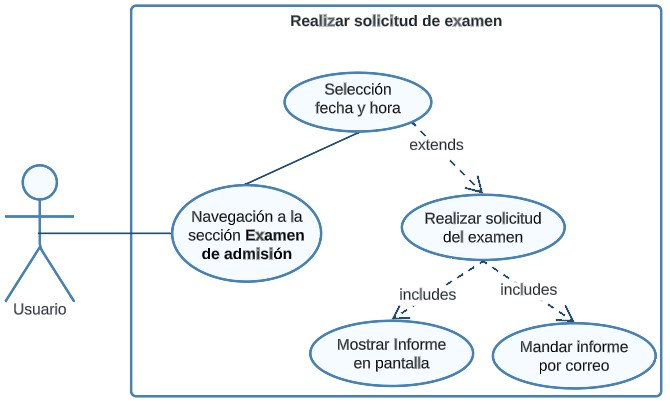
\includegraphics[width=\textwidth]{./img/casousoSolicitarExamen.jpg}}
  \caption{Diagrama de caso de uso: Realizar solicitud de examen}
  \label{fig:diagRealizarsolicitud}
\end{figure}

\subsection{Caso de uso: Simular notas de exámenes}

\begin{tcolorbox}[colback=white, colframe=black, rounded corners]
  {\Large \textbf{Caso de uso: Simulación de notas de examen}} \\
  {\large Actor: Administrador} \vspace*{0.5cm} \\
  {{\large \textbf{Precondiciones}} \\
  1. El administrador ha ingresado al sistema. \\
  2. Hay solicitudes de examen para el período actual.
  } \vspace*{0.5cm} \\
  {{\large \textbf{Flujo principal}} \\
  1. El administrador navega a la sección de "Solicitudes de Examen". \\
  2. El sistema muestra las solicitudes del período actual. \\
  3. Opcionalmente, el administrador puede filtrar las solicitudes según la carrera. \\
  4. El administrador selecciona las solicitudes a las cuales desea asignarles notas. \\
  5. El administrador hace clic en el botón "Simular notas". \\
  6. El sistema genera y asigna una nota aleatoria de admisión a las solicitudes seleccionadas. \\
  7. Se muestra una confirmación de que las notas han sido asignadas.
  } \vspace*{0.5cm} \\
  {{\large \textbf{Flujo alternativo}} \\
  3a. No se realiza ningún filtrado.
  \begin{itemize}
    \item El administrador ve todas las solicitudes sin filtrar por carrera.
  \end{itemize}
  5a. Ninguna solicitud es seleccionada.
  \begin{itemize}
    \item El sistema muestra un mensaje de error indicando que se deben seleccionar solicitudes.
  \end{itemize}
  7a. Error al simular notas.
  \begin{itemize}
    \item El sistema muestra un mensaje de error indicando que no se pudieron asignar las notas.
  \end{itemize}
}
\end{tcolorbox}

\begin{figure}[H]
  \centering
  \frame{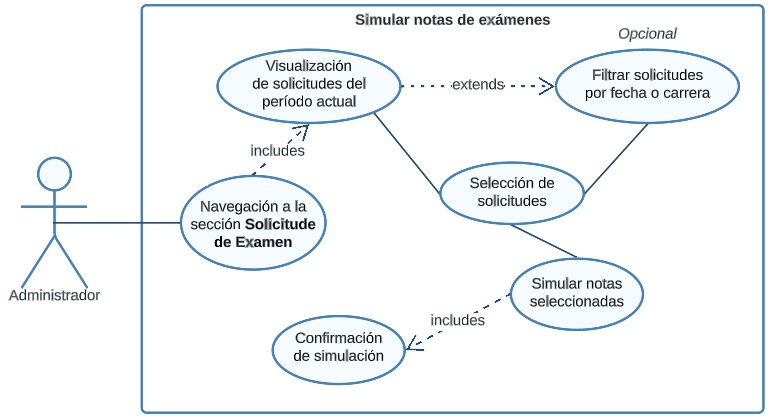
\includegraphics[width=\textwidth]{./img/casousoSimularNotas.jpg}}
  \caption{Diagrama de caso de uso: Simular notas de exámenes}
  \label{fig:diagusoSimularNotas}
\end{figure}

\subsection{Caso de uso: Asignar estados de solicitudes}

\begin{tcolorbox}[colback=white, colframe=black, rounded corners]
  {\Large \textbf{Caso de uso: Asignación de Estado a Solicitudes}} \\
  {\large Actor: Administrador} \vspace*{0.5cm} \\
  {{\large \textbf{Precondiciones}} \\
  1. El administrador ha ingresado al sistema. \\
  2. Existen solicitudes con notas asignadas.
  } \vspace*{0.5cm} \\
  {{\large \textbf{Flujo principal}} \\
  1. El administrador navega a la sección de "Solicitudes con Notas". \\
  2. El sistema muestra todas las solicitudes que tienen notas asignadas. \\
  3. Opcionalmente, el administrador puede filtrar las solicitudes. \\
  4. Selecciona las solicitudes y les asigna un estado (admitido, en proceso, rechazado). \\
  5. El sistema confirma la actualización del estado de las solicitudes seleccionadas.
  } \vspace*{0.5cm} \\
  {{\large \textbf{Flujo alternativo}} \\
  4a. Ninguna solicitud es seleccionada.
  \begin{itemize}
    \item El sistema muestra un mensaje indicando que se deben seleccionar solicitudes para actualizar el estado.
  \end{itemize}
  5a. Error al actualizar el estado.
  \begin{itemize}
    \item El sistema muestra un mensaje de error indicando que no se pudo actualizar el estado de las solicitudes.
  \end{itemize}
}
\end{tcolorbox}

\begin{figure}[H]
  \centering
  \frame{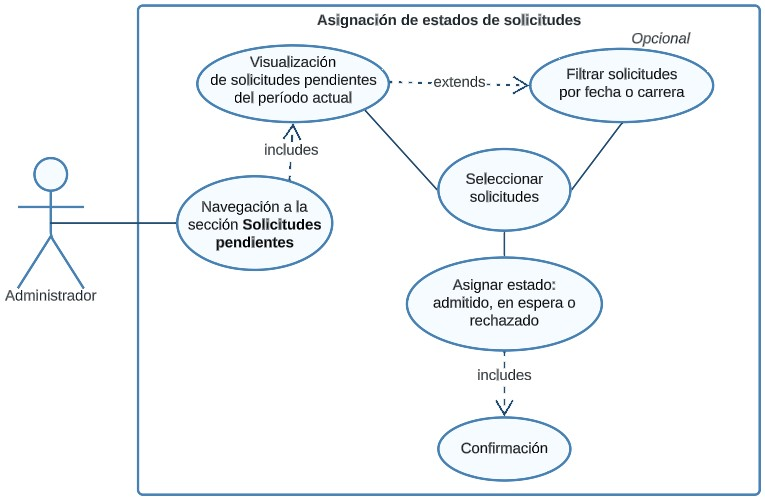
\includegraphics[width=\textwidth]{./img/casousoAsignarEstadoExamen.jpg}}
  \caption{Diagrama de caso de uso: Asignar estado a solicitud}
  \label{fig:diagusoAsignarEstadoExamen}
\end{figure}

\subsection{Caso de uso: Generar reportes}

\begin{tcolorbox}[colback=white, colframe=black, rounded corners]
  {\Large \textbf{Caso de uso: Generación de Reportes}} \\
  {\large Actor: Administrador, Solicitante} \vspace*{0.5cm} \\
  {{\large \textbf{Precondiciones}} \\
  1. El administrador/solicitante ha ingresado al sistema. \\
  2. Existen datos de exámenes de admisión por lo menos de un año.
  } \vspace*{0.5cm} \\
  {{\large \textbf{Flujo principal}} \\
  1. El administrador/solicitante navega a la sección de ``Solicitudes pendientes''. \\
  2. El administrador selecciona un año de aplicación de examen de admisión. \\
  3. El administrador selecciona un tipo de reporte. \\
  4. El administrador solicita al sistema generar el reporte. \\
  5. El sistema muestra una visualización preliminar del reporte. \\
  } \vspace*{0.5cm} \\
  {{\large \textbf{Flujo alternativo}} \\
  4a. Error al generar el reporte.
  \begin{itemize}
    \item El sistema muestra un mensaje de error indicando que no se pudo generar el reporte.
  \end{itemize}
}
\end{tcolorbox}

\begin{figure}[H]
  \centering
  \frame{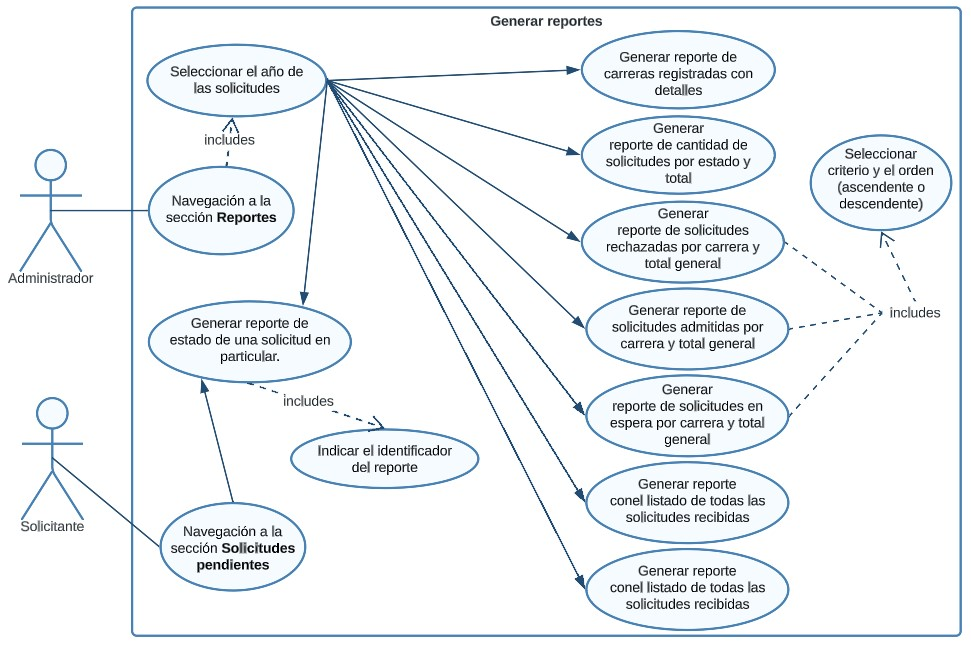
\includegraphics[width=\textwidth]{./img/casousoDescargarInforme.jpg}}
  \caption{Diagrama de caso de uso: Generar reportes de solicitudes}
  \label{fig:diagusoGenerarReportes}
\end{figure}

\subsection{Caso de uso: Gestionar cortes de carreras}
\begin{tcolorbox}[colback=white, colframe=black, rounded corners]
  {\Large \textbf{Caso de uso: Gestión de cortes de carrera}} \\
  {\large Actor: Administrador} \vspace*{0.5cm} \\
  {{\large \textbf{Precondiciones}} \\
  1. El administrador ha ingresado al sistema. \\
  2. Existen carreras registradas en el sistema.
  } \vspace*{0.5cm} \\
  {{\large \textbf{Flujo principal}} \\
  1. El administrador consulta la lista de carreras. \\
  2. El administrador busca una carrera por nombre usando el buscador. \\
  3. El administrador selecciona una carrera de la lista. \\
  4. El administrador modifica la nota mínima de admisión, la cantidad máxima de admitidos por año o ambos. \\
  5. El sistema valida la información ingresada. \\
  6. El sistema solicita confirmación al administrador sobre los cambios realizados. \\
  7. El administrador confirma y el sistema guarda los cambios.
  } \vspace*{0.5cm} \\
  {{\large \textbf{Flujo alternativo}} \\
  5a. Información ingresada no válida.
  \begin{itemize}
    \item El sistema muestra un mensaje de error.
    \item El administrador puede corregir la información y reintentar.
  \end{itemize}
  6a. El administrador no confirma los cambios.
  \begin{itemize}
    \item Se cancelan los cambios y se retorna al estado anterior.
  \end{itemize}
}
\end{tcolorbox}

\begin{figure}[H]
  \centering
  \frame{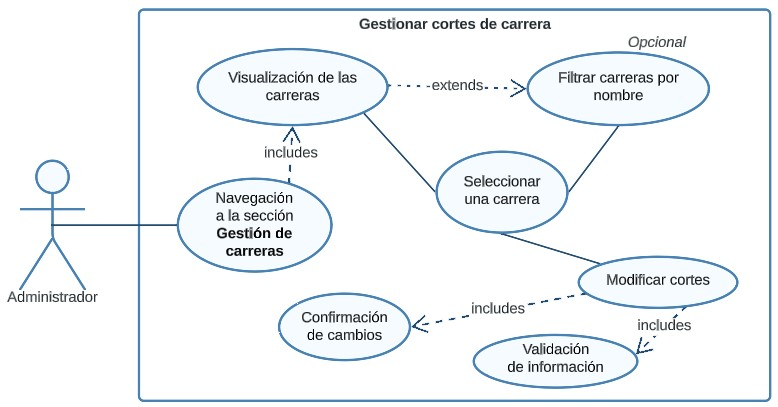
\includegraphics[width=\textwidth]{./img/casousoGestionCarrera.jpg}}
  \caption{Diagrama de caso de uso: Gestión de cortes de carrera}
  \label{fig:diagusoGestionCarreras}
\end{figure}

\section{Vista lógica}

\subsection{Modelo de negocios}

\begin{figure}[H]
  \centering
  \frame{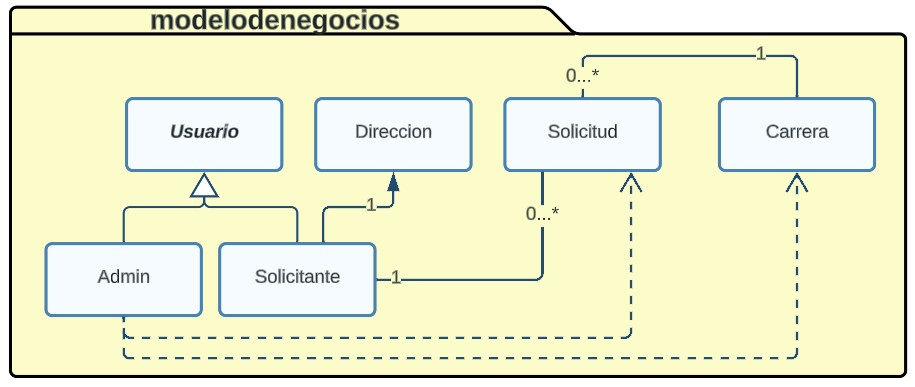
\includegraphics[width=0.7\textwidth]{./img/modelonegResumen.jpg}}
  \caption{Modelo de negocios resumido}
  \label{fig:ModeloNegResumido}
\end{figure}

Primero, el sistema requiere de un proceso de registro e inicio de sesión. Se deben considerar tanto a las usuarios \textit{administradores} y a los usuarios ``normales''. Para ello vamos a definir primero una clase abstracta denominada \textit{Usuario}.

\subsubsection*{Clase Abstracta Usuario}

\begin{wrapfigure}[3]{l}{0.3\textwidth}
  \frame{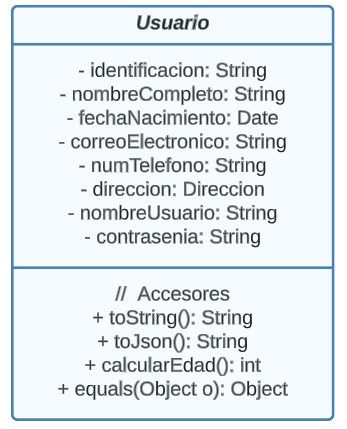
\includegraphics[width=0.3\textwidth]{./img/ClaseUsuario.jpg}}
  \caption{Clase Usuario}
  \label{fig:mi_etiqueta}
\end{wrapfigure}

Definimos una clase Usuario común con las características más básicas que tienen usuarios de esta vamos a derivar las clases \textit{Admin} y \textit{Solicitante}. 

\newpage

\subsubsection*{Clases Administrador, Solicitante y Dirección}

\begin{figure}[H]
  \centering
  \frame{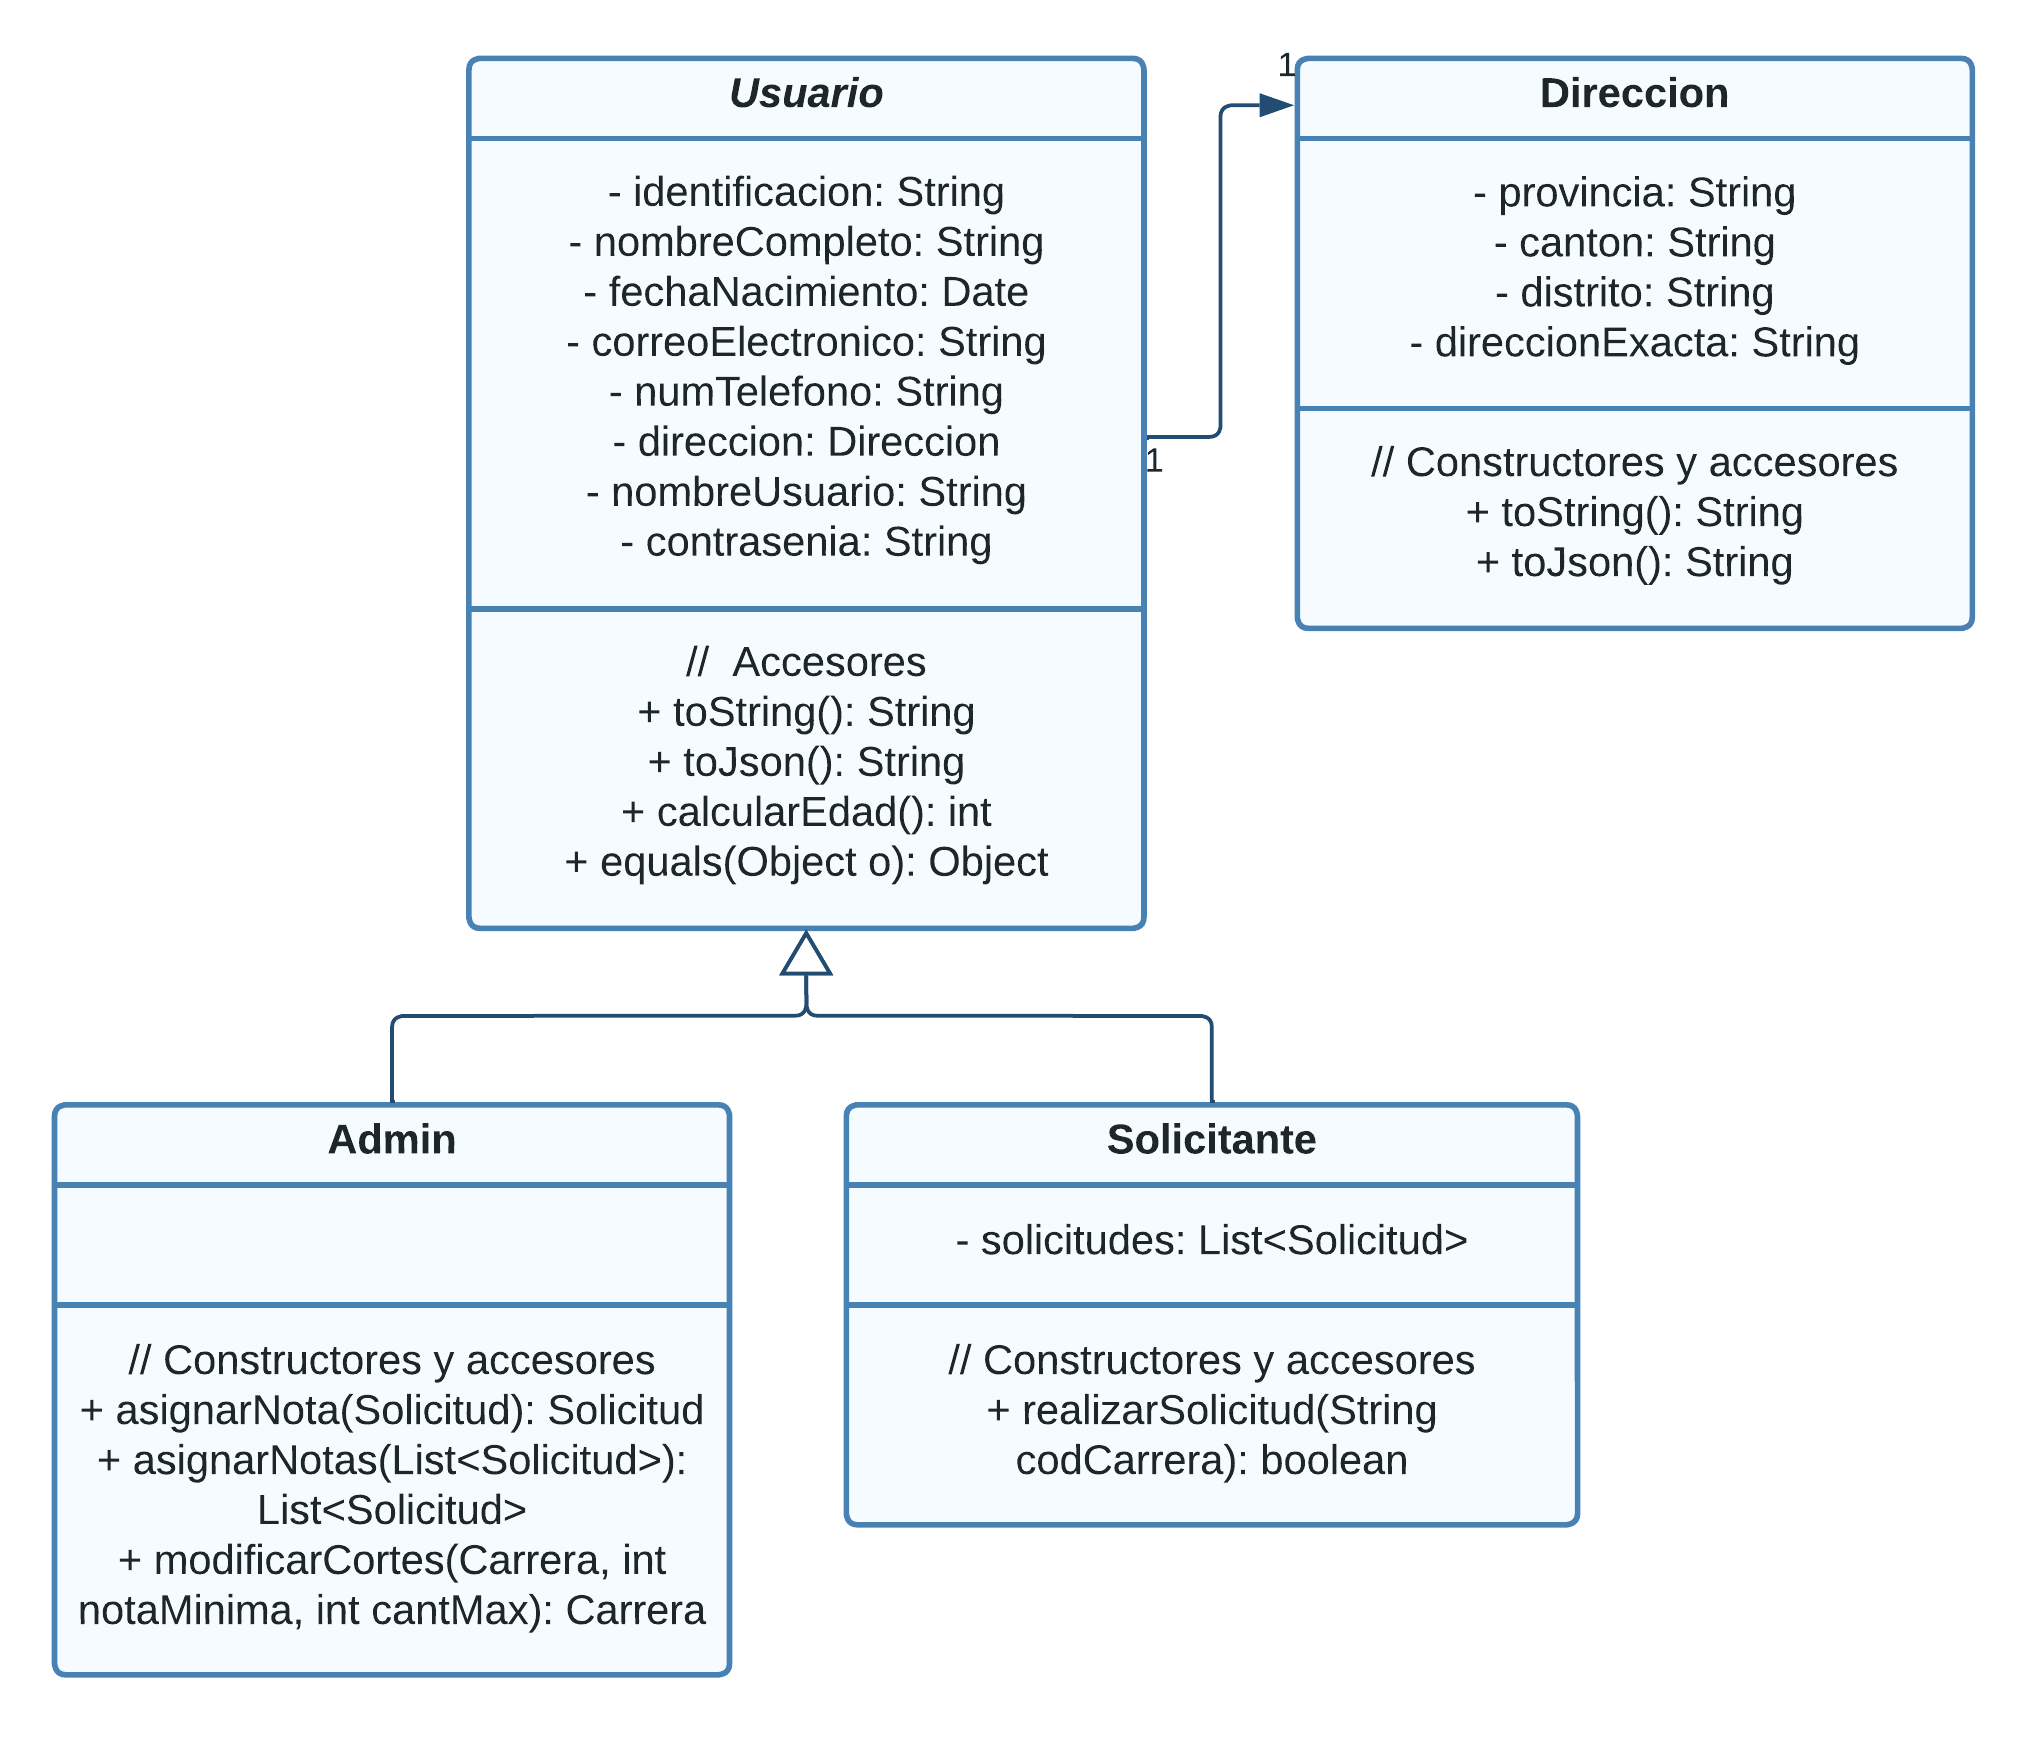
\includegraphics[width=0.7\textwidth]{./img/ClaseUsuarioDetalle.png}}
  \caption{Clases Admin, Solicitante y Dirección}
  \label{fig:ClaseAdminSoliDir}
\end{figure}

Se definió la clase \textit{Dirección} por separado, y se definieron las clases de \textit{Admin} y \textit{Solicitante} en donde varían principalmente en los métodos que pueden realizar. Según la especificación el
\begin{itemize}
  \item \textbf{Admin} puede asignar notas, nada más que esto se realizará de forma aleatoria; puede cambiar los cortes de una carrera, que implica que puede modificar la \textit{nota mínima para ingresar} y la \textit{capacidad máxima que se puede aceptar} para una carrera.
  \item \textbf{Solicitante} puede realizar la solicitud para realizar el examen de admisión indicando el código de la carrera.
\end{itemize}

La clase \textit{Dirección} es muy trivial y no se va a detallar.

\concept{Lista de solicitudes}{
  Los solicitantes tienen una lista de las solicitudes que han realizado en la plataforma. Eso se agregó considerando la propuesta de mantener la escalabilidad del sistema mencionada anteriormente.
}

\subsubsection*{Clases Solicitud y Carrera}

\begin{figure}[H]
  \centering
  \frame{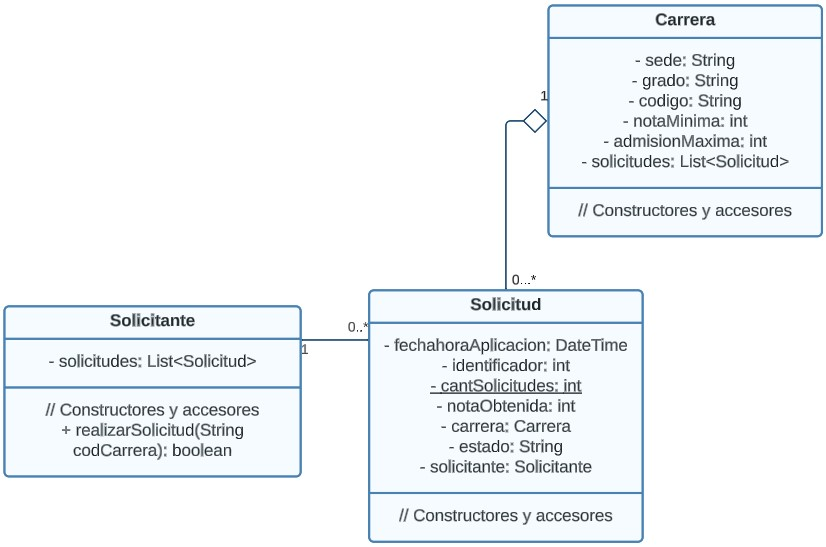
\includegraphics[width=0.7\textwidth]{./img/ClaseSolicitudCarrera.jpg}}
  \caption{Clases Solicitud y Carrera}
  \label{fig:ClaseSoliCarr}
\end{figure}

Por último, tenemos las clases de Solicitud y Carrera. No tienen ninguna funcionalidad en específico, el administrador se encargará de acceder a las instancias de estos objetos.

\concept{Justificación}{
  Un solicitante puede tener varias solicitudes y además, una carrera estará agregada por varias solicitudes. Estas relaciones facilitarán la consulta para los servicios solicitades del sistema.
}

El sistema completo con más detalle se visualizaría en la siguiente figura.

\begin{figure}[H]
  \centering
  \frame{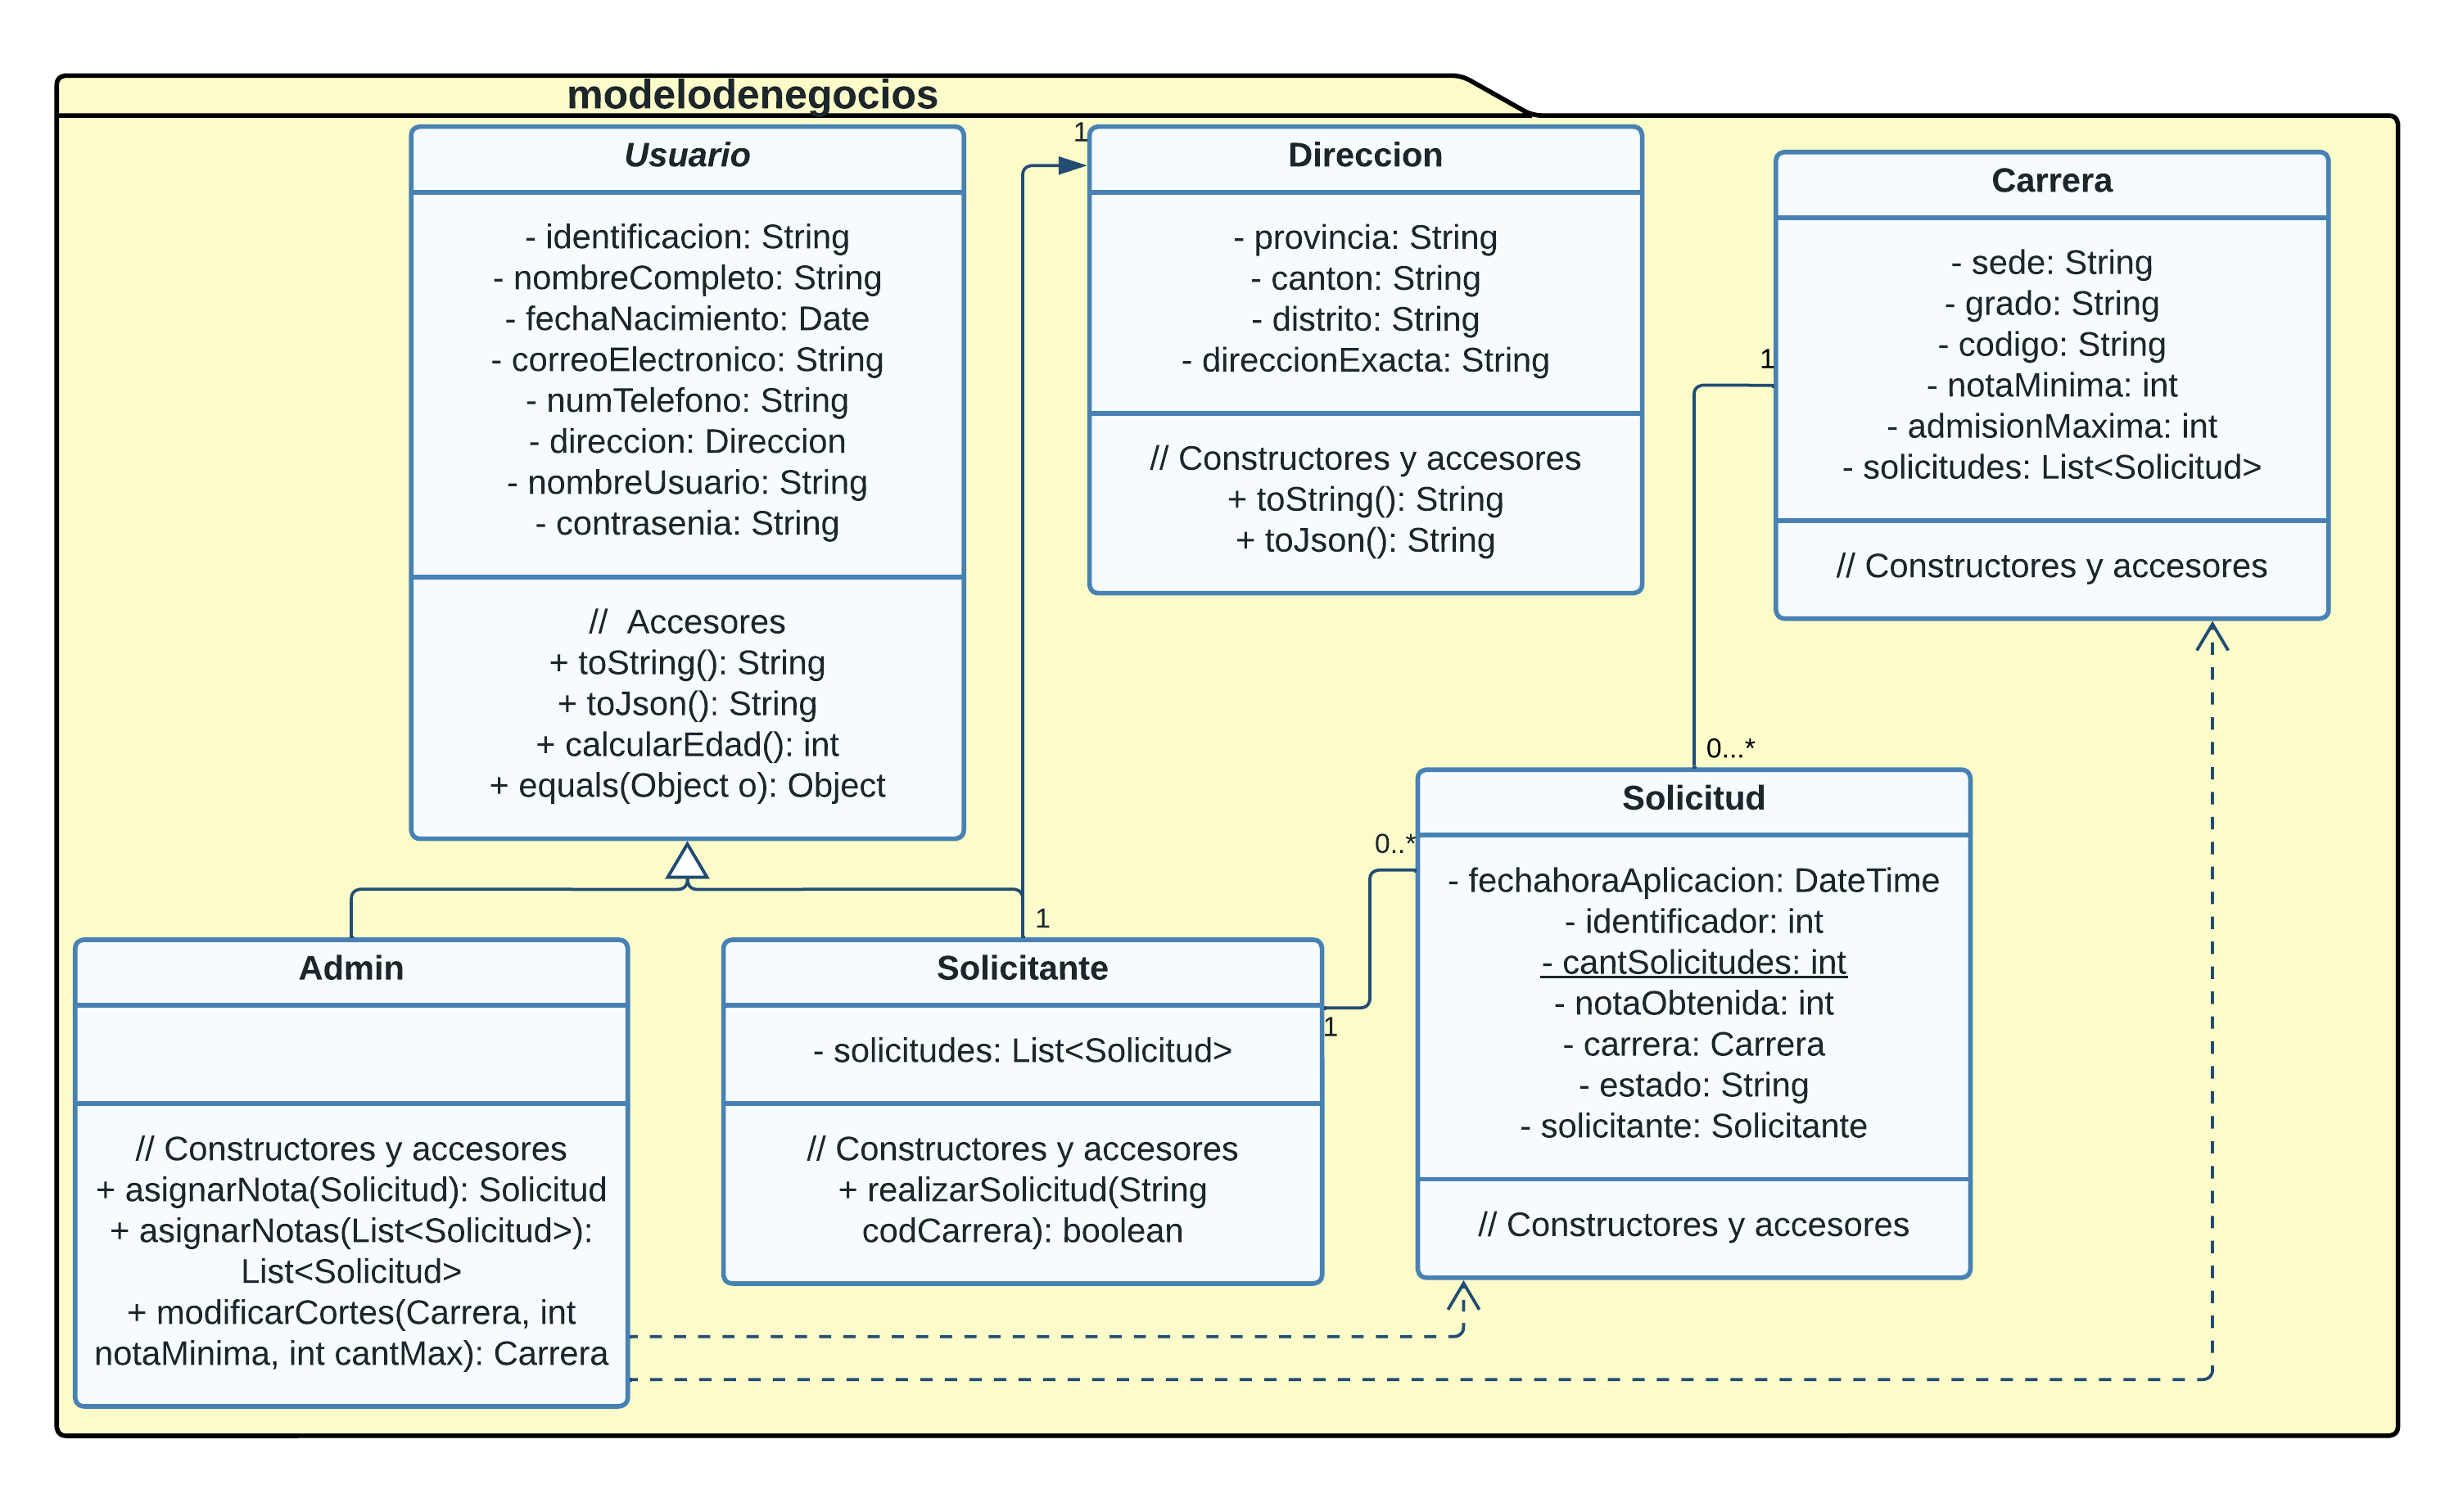
\includegraphics[width=0.8\textwidth]{./img/modelonegDetallado.png}}
  \caption{Modelo de negocios detallado}
  \label{fig:ModeloNegDetallado}
\end{figure}

\subsection{Controladores y Vistas}

Como se mencionó anteriormente, la arquitectura del sistema será utilizando el patrón \textit{modelo-vista-controlador (MVC)}. Además, se utilizará el paquete de \textit{Data Access Object (DAO)} para la estructuración de los datos obtenidos desde la base de datos y moldearlos apropiadamente con nuestro modelo de negocios. La organización de la lógica del sistema se puede representar con el siguiente diagrama:

\begin{figure}[H]
  \centering
  \frame{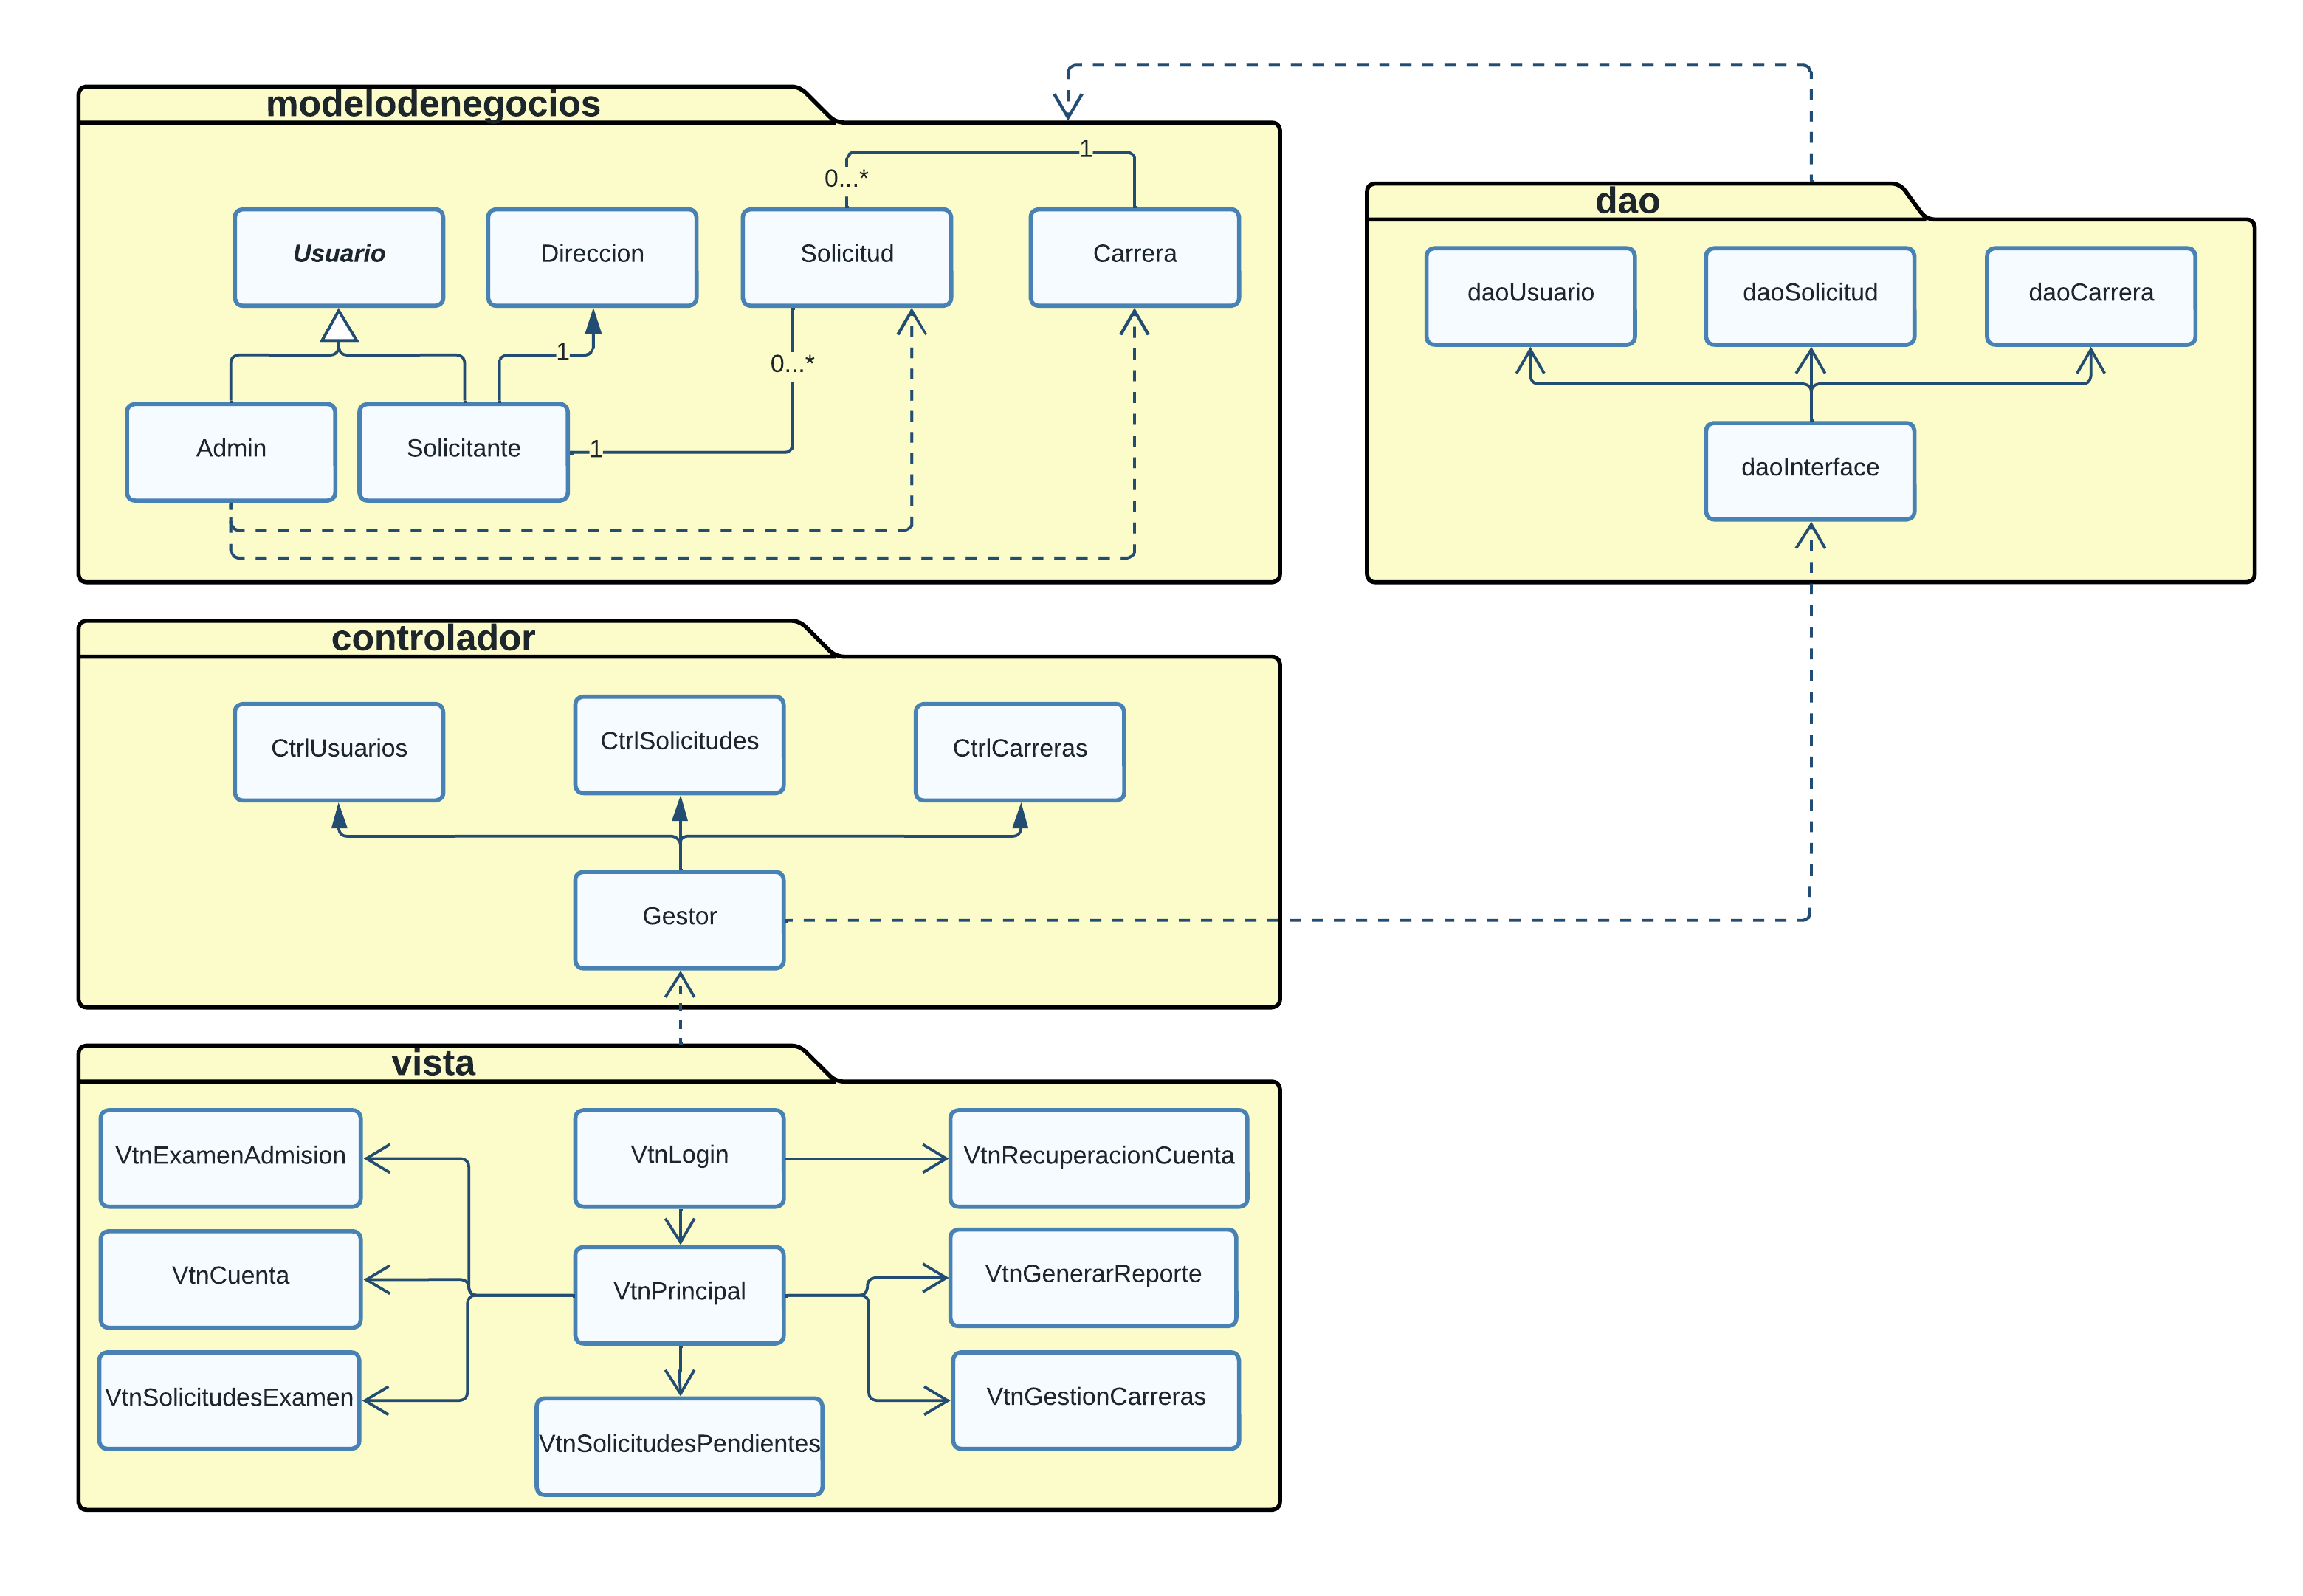
\includegraphics[width=0.8\textwidth]{./img/modeloResumidoCompleto.png}}
  \caption{Arquitectura resumida}
  \label{fig:arqResumidaSinDetalle}
\end{figure}

Los \textbf{controladores} se encargarán del apartado lógico de manipulación de datos. Recordando que:
\begin{itemize}
  \item Un administrador puede modificar información de las carreras.
  \item Un administrador puede ``simular'' notas de exámenes (actualizando las solicitudes).
  \item Un administrador puede cambiar el estado de una solicitud como: \textbf{en proceso, rechazada o admitida}.
  \item Los usuarios pueden realizar solicitudes de exámenes de admisión una vez por año.
\end{itemize}

\subsection{Propuestas de vistas}

A continuación se presenta un modelo preliminar de las vistas en modo \textit{Solicitante}. La ilustrar la idea principal del modelo propuesto para los solicitantes, las vistas del modo \textit{administrador} no serán incluidas.

\subsubsection*{Ventana Login}

\begin{figure}[H]
  \centering
  \frame{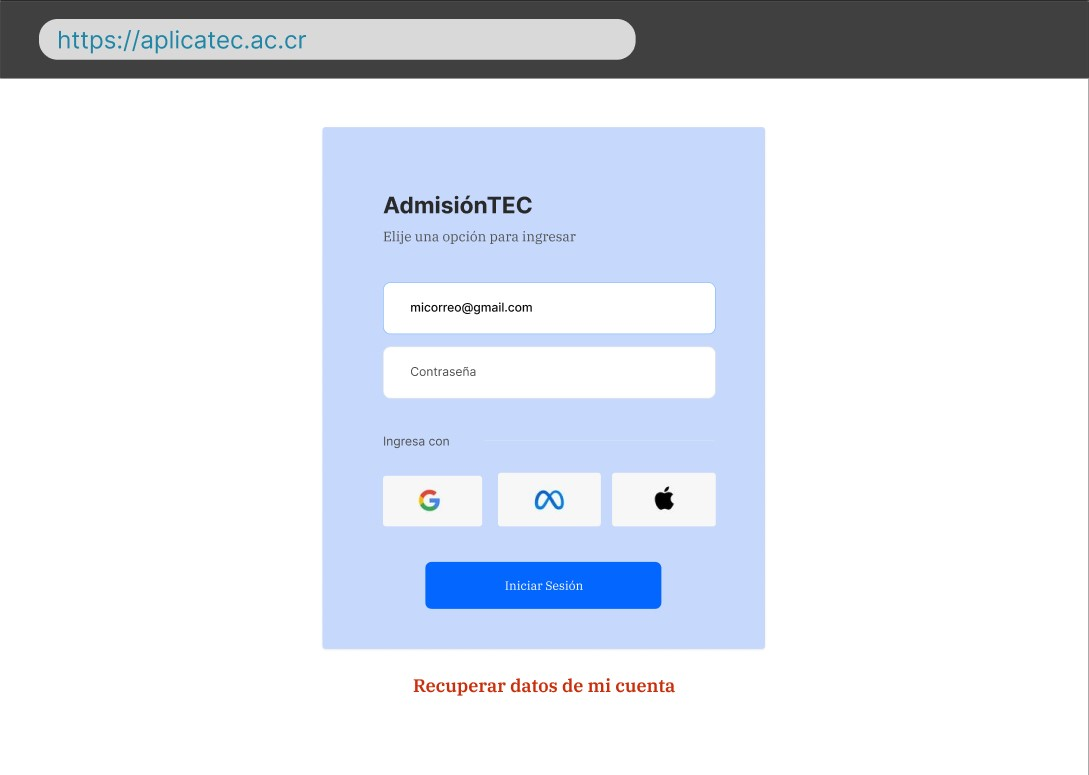
\includegraphics[width=0.8\textwidth]{./img/vista01Login.jpg}}
  \caption{Ventana Login}
  \label{fig:vtnLogin}
\end{figure}

\subsubsection*{Ventana principal}

\begin{figure}[H]
  \centering
  \frame{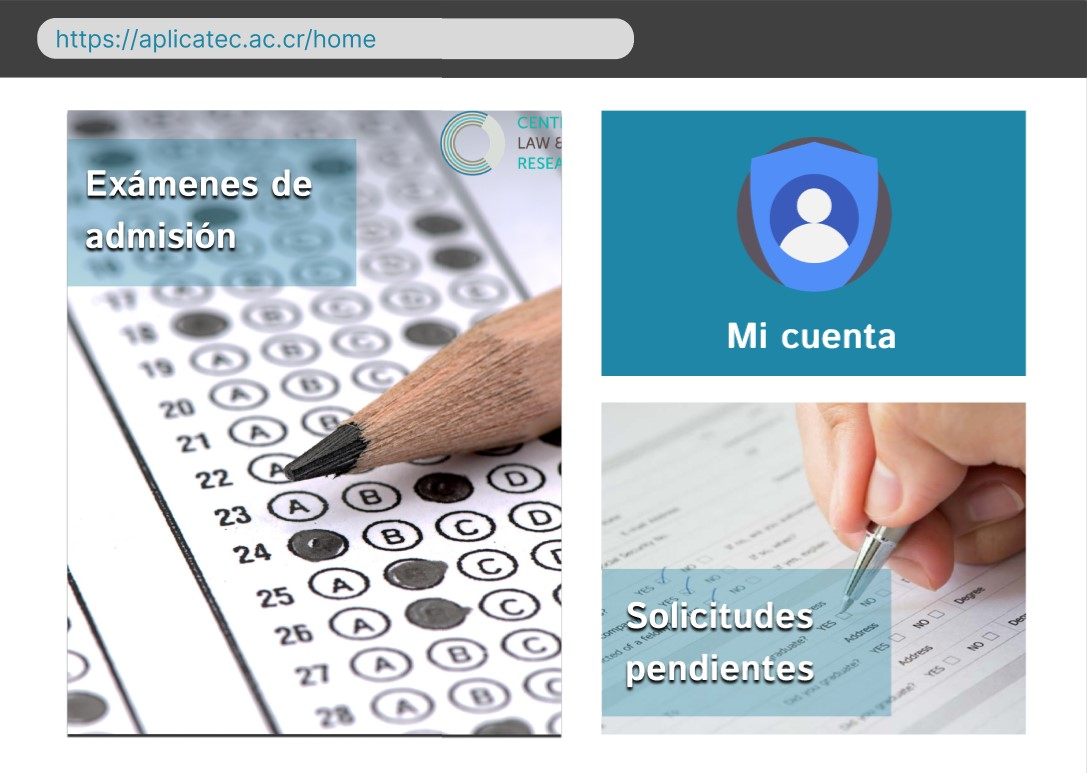
\includegraphics[width=0.8\textwidth]{./img/vista02PrincipalUsuario.jpg}}
  \caption{Ventana principal}
  \label{fig:vtnPrincipal}
\end{figure}

\subsubsection*{Ventana para solicitar hacer el examen}

\begin{figure}[H]
  \centering
  \frame{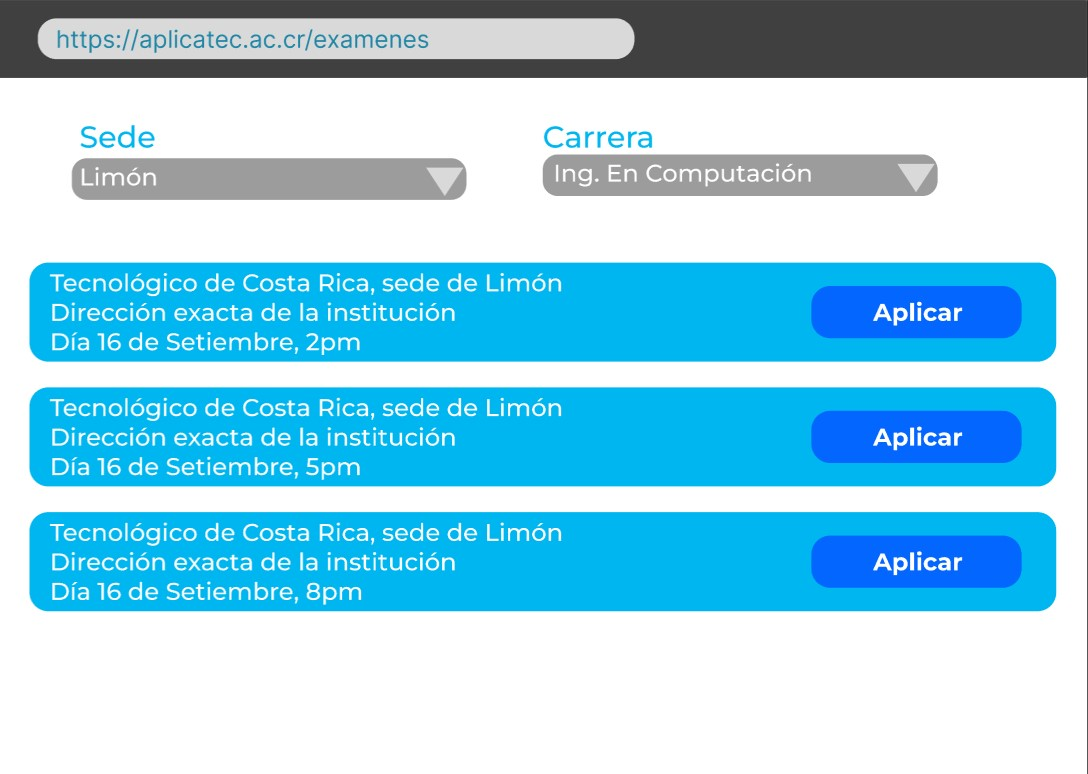
\includegraphics[width=0.8\textwidth]{./img/vista03ExamenesUsuario.jpg}}
  \caption{Ventana de citas para el examen de admisión}
  \label{fig:vtnExamenesUsuario}
\end{figure}

\section{Vista de deployment}

A continuación se ilustrará una descripción breve de la configuración del deployment del sistema. En esta aplicación se asume que hay una base de datos externa que tiene información correspondiente a las carreras, en nuestro modelo definimos una base de datos que albergará la información de los solicitantes y sus respectivas solicitudes.

Además, se integrará un módulo para la gestión de correos electrónicos considerando que el sistema notificará a los usuarios cuando realicen las solicitudes y cuando se les notifique su nota del examen de admisión al cuál aplicaron. Junto con un módulo de validación de cuentas de forma segura, considerando que se maneja información sensible en este sistema.

\begin{figure}[H]
  \centering
  \frame{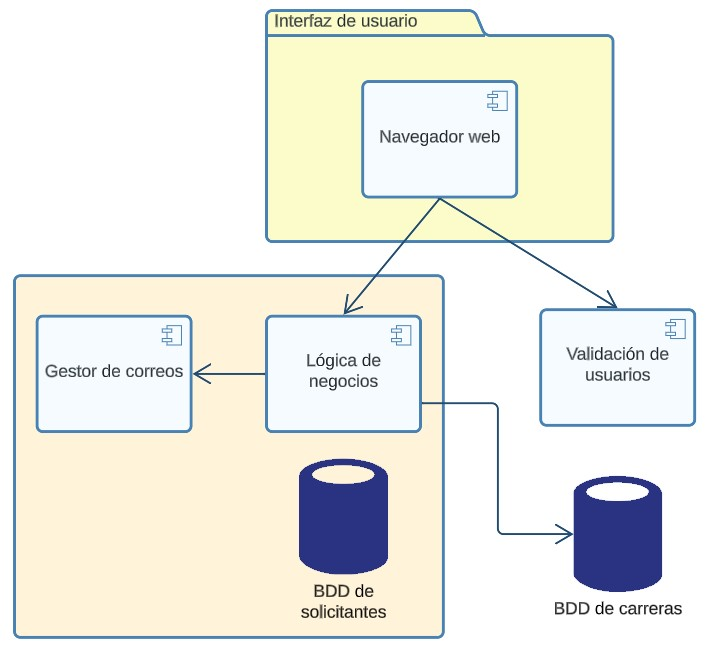
\includegraphics[width=0.8\textwidth]{./img/deployment.jpg}}
  \caption{Resumen del deployment de la aplicación}
  \label{fig:deployment}
\end{figure}

\section{Calidad}

A continuación se mencionan algunos atributos importantes y puntuales referentes a la calidad del sistema:

\begin{itemize}
  \item El sistema deberá ser capaz de manejar hasta 10000 solicitudes de forma simultánea sin degradar el rendimiento. Para efectos de costo, se consideran nada más los períodos clave (durante los procesos de admisión del año).
  \item El sistema deberá ser compatible con las bases de datos MySQL (se asume que la base de datos de las carreras este motor de base de datos).
  \item El sistema debe ser robusto, la seguridad es importante para evitar accesos no autorizados y resguardar la información sensible de la población. Además de evitar la alteración indebida de datos.
  \item El sistema debe estar disponible 24/7. No debe tener más de un 5\% de inactividad.
  \item La interfaz debe ser fácil de usar. Además, se contará con un sistema guía para las personas que estén ingresando a la aplicación por primera vez.
  \item El soporte deberá estar integrado al sistema, abierto y disponible para las consultas de los usuarios registrados.
\end{itemize}

\section{Tamaño y rendimiento}

Los principales requisitos de tamaño y tiempo se definen:

\begin{itemize}
  \item El sistema deberá proporcionar acceso a la base de datos con no más de 8 segundos de latencia.
  \item El sistema deberá ser capaz de completar el 85\% de todas las transacciones dentro de 1.5 minutos.
  \item La parte del cliente requerirá menos de 25 MB de espacio en disco y 40MB de RAM.
\end{itemize}

\end{document}
